%!TEX TS-program = xelatex
%!TEX encoding = UTF-8 Unicode
\documentclass[reqno ,12pt]{amsart}
\usepackage[foot]{amsaddr}
\usepackage{graphicx}
\usepackage[usenames,dvipsnames]{xcolor}
\usepackage[paperwidth=7in,paperheight=10in,text={5in,8in},left=1in,top=1in,headheight=0.25in,headsep=0.4in,footskip=0.4in]{geometry}
%\usepackage{mathtools}
\usepackage{subfigure}
\usepackage{lineno}
\usepackage{natbib} %this allows for styles in referencing
%\bibpunct[, ]{(}{)}{,}{a}{}{,}
\DeclareMathOperator{\var}{var}
\DeclareMathOperator{\cov}{cov}
\DeclareMathOperator{\E}{E}
\DeclareMathOperator{\logit}{logit}

\synctex=1

\newcommand*\patchAmsMathEnvironmentForLineno[1]{%
  \expandafter\let\csname old#1\expandafter\endcsname\csname #1\endcsname
  \expandafter\let\csname oldend#1\expandafter\endcsname\csname end#1\endcsname
  \renewenvironment{#1}%
     {\linenomath\csname old#1\endcsname}%
     {\csname oldend#1\endcsname\endlinenomath}}%
\newcommand*\patchBothAmsMathEnvironmentsForLineno[1]{%
  \patchAmsMathEnvironmentForLineno{#1}%
  \patchAmsMathEnvironmentForLineno{#1*}}%
\AtBeginDocument{%
\patchBothAmsMathEnvironmentsForLineno{equation}%
\patchBothAmsMathEnvironmentsForLineno{align}%
\patchBothAmsMathEnvironmentsForLineno{flalign}%
\patchBothAmsMathEnvironmentsForLineno{alignat}%
\patchBothAmsMathEnvironmentsForLineno{gather}%
\patchBothAmsMathEnvironmentsForLineno{multline}%
}

%\usepackage{lmodern}
%\usepackage{unicode-math}
\usepackage{mathspec}
\usepackage{xltxtra}
\usepackage{xunicode}
\defaultfontfeatures{Mapping=tex-text}
%\setsansfont[Scale=MatchLowercase,Mapping=tex-text]{Helvetica}
%\setmonofont[Scale=0.85]{Bitstream Vera Sans Mono}
\setmainfont[Scale=1,Ligatures={Common}]{Adobe Caslon Pro}
\setromanfont[Scale=1,Ligatures={Common}]{Adobe Caslon Pro}
\setmathrm[Scale=1]{Adobe Caslon Pro}
\setmathfont(Digits,Latin)[Numbers={Lining,Proportional}]{Adobe Caslon Pro}

\definecolor{linenocolor}{gray}{0.6}
\renewcommand\thelinenumber{\color{linenocolor}\arabic{linenumber}}

\usepackage{fix-cm}

%\usepackage{hanging}

\setcounter{totalnumber}{1}

\newcommand{\mr}{\mathrm}
\newcommand{\tsc}[1]{\text{\textsc{#1}}}

\begin{document}

\title{Estimating Extra-Pair Paternity in a Heterogenous Sample}
\author{Richard McElreath}
\address{Department of Human Behavior, Ecology and Culture, Max Planck Institute for Evolutionary Anthropology, Leipzig, Germany}
\email{richard\_mcelreath@eva.mpg.de}

%\date{\today}

\maketitle

{\vspace{-6pt}\footnotesize\begin{center}\today\end{center}\vspace{12pt}}

\linenumbers
\modulolinenumbers[3]


%begin{abstract}{
%\noindent {\small
%abstract}
%\end{abstract}


The sample comprises mothers with varying numbers of both children and husbands. In principle, each mother and mother-husband pair could have a unique extra-pair paternity (EPP) rate. Estimates of both the average rate and the variation among mothers and mother-husband pairs can be constructed with a multilevel analysis.

\subsection*{Statistical model}

Let $y_i \in \{0,1\}$ be the EPP status of child $i$. Each child has a corresponding mother with index $\textsc{mom}[i]$ and a dyad comprising the mother and the child's social father with index $\textsc{dyad}[i]$. Then the probability of $y_i$ is given by:
\begin{align*}
	y_i &\sim \mathrm{Bernoulli}(p_i)\\
	\logit p_i &= \alpha + z_{\textsc{mom}[i]} \sigma + x_{\textsc{dyad}[i]} \tau
\end{align*}
where $\alpha$ is the population average, the vector $z$ contains standardized varying effects for each mother, $\sigma$ is the standard deviation among mothers, $x$ contains standardized varying effects for each dyad, and $\tau$ is the standard deviation among dyads.

The model uses a non-centered parameterization, but is in fact an ordinary multi-level model. The priors are:
\begin{align*}
	\alpha &\sim \mr{Normal}(0,1.5)\\
	z_j &\sim \mr{Normal}(0,1)\\
	x_k &\sim \mr{Normal}(0,1)\\
	\sigma &\sim \text{Half-Normal}(0,1)\\
	\tau &\sim \text{Half-Normal}(0,1)
\end{align*}
The $\mr{Normal}(0,1.5)$ prior for $\alpha$ establishes a uniform prior on the probability scale and Half-Normal(0,1) indicates a normal distribution defined only on positive reals.

\subsection*{Measurement error}

A complication in this analysis is that there is as much as 5\% false assignment of paternity. Failing to account for this would artificially inflate our estimate of EPP. We incorporate false-positives into our model by using a mixture likelihood. Given false-positive probability $f$, the probability of observing a paternity assignment $y_i=1$ is:
\begin{align*}
	\Pr( y_i=1 | p_i ) = (1-f\,) p_i + f\, (1 - p_i)
\end{align*}
Since false negatives are extremely unlikely in our analysis, the probability of observing $y_i=0$ remains unchanged:
\begin{align*}
	\Pr( y_i=0 | p_i ) = 1 - p_i
\end{align*}

\subsection*{Implementation}

We implemented the model in Stan 2.19 (\texttt{mc-stan.org}), a library for Bayesian model construction and fitting. A copy of the script is available at \texttt{LINK}. We drew 8000 samples from 4 chains. All R-hat values were less than 1.01, and there were no divergent transitions or other signs of biased posterior exploration. We show the trace plots for the hyper-parameters and a selection of the varying effects on the next page. We also show the same traces as rank histograms (https://arxiv.org/abs/1903.08008), which make it much easier to spot problems with chains. Healthy chains, like these, should be relatively uniform.

\begin{figure}[p]
\begin{center}
	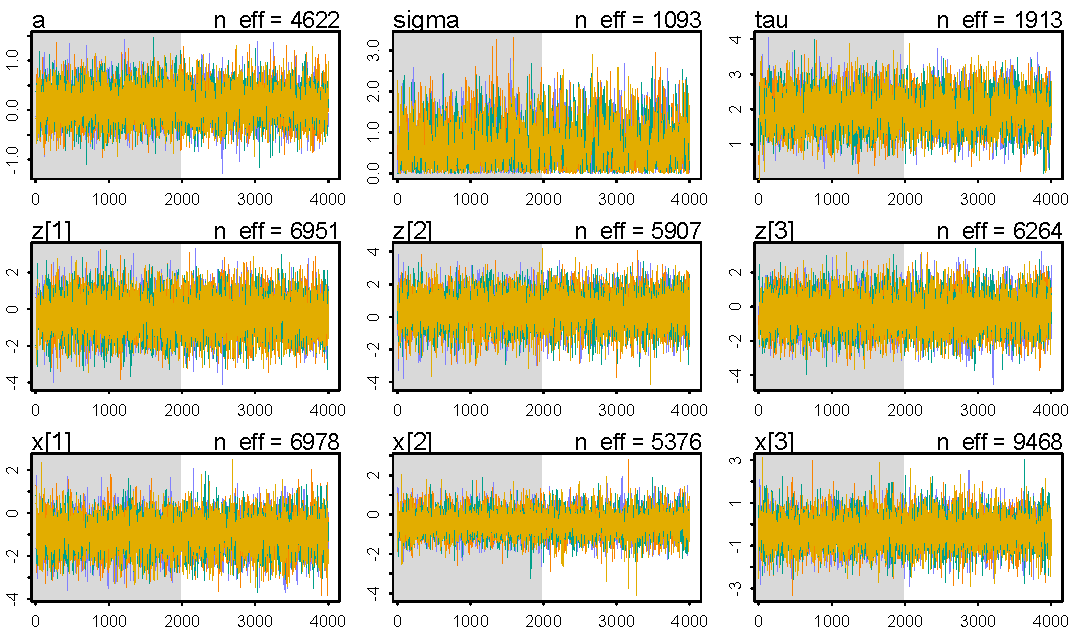
\includegraphics[scale=0.7]{trace.pdf}
	\hrule
	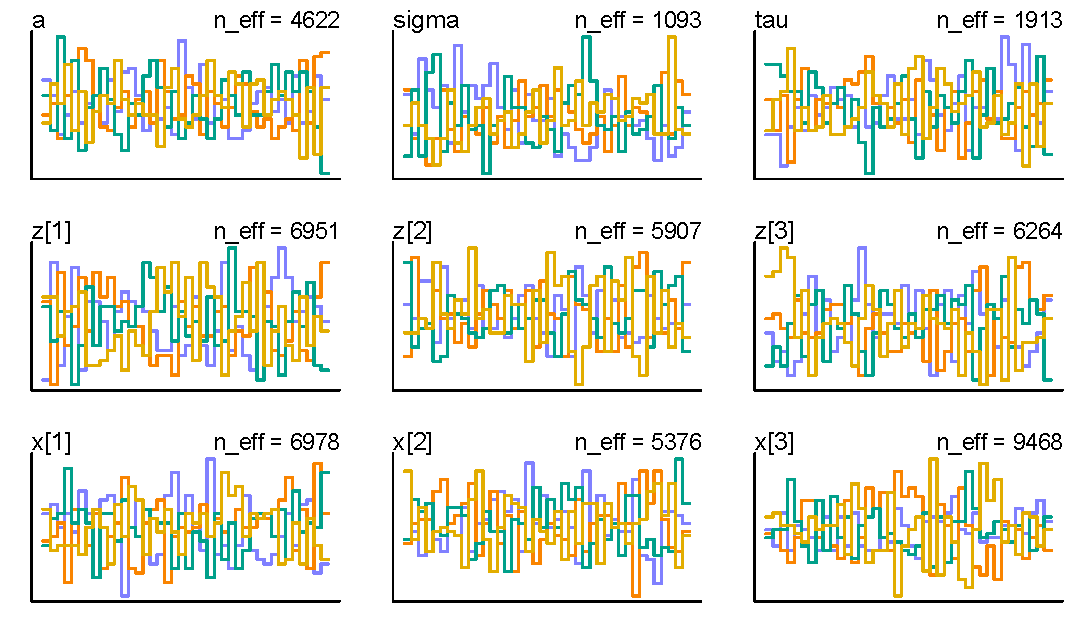
\includegraphics[scale=0.7]{trank.pdf}
\caption{Trace plots (top) and rank histograms (bottom) for the model that clusters by mother and mother-husband dyad.}
\label{fig_traces}
\end{center}
\end{figure}

The marginal posterior distributions for $\alpha$, $\sigma$, and $\tau$ are summarized below.
\begin{verbatim}
       mean   sd  5.5% 94.5% n_eff Rhat
a     -0.07 0.36 -0.63  0.51  6422    1
sigma  0.75 0.55  0.07  1.75  1216    1
tau    2.01 0.54  1.18  2.89  2325    1
\end{verbatim}
On the probability scale, $\alpha$ implies an average posterior EPP rate with mean 0.48 and 95\% credible interval from 0.32 to 0.66. Note that there is more variation among dyads ($\tau$) than among mothers ($\sigma$). This implies that features of specific pairings explain EPP variation more than features of specific women.

The posterior distribution EPP rate is plotted below in red, against both the prior (dashed) and the naive posterior rate from ignoring clustering by mothers and mother-father dyads (black). 
We also considered models with no clustering (the black density in the above figure), with clustering only by mother, and clustering only by dyad. All models with clustering produce similar inferences. Code for each, together with WAIC model comparison, can be found in the script (LINK). 
For comparison, models which do not include potential false-positives are shown in lighter colors.

\begin{center}
	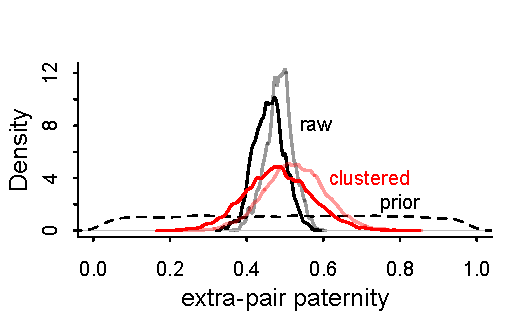
\includegraphics[scale=1]{EPP_posterior.pdf}
\end{center}



%\clearpage
%\bibliographystyle{newapa}
%\bibliography{covert}

\end{document}
